\documentclass[twoside]{article}

\usepackage{ustj}
\usepackage{tikz}
\usepackage{pgfplots}

\addbibresource{mss.bib}

\newcommand{\authorname}{Trent Steen}
\newcommand{\authorpatp}{\patp{hanfel-dovned}}
\newcommand{\affiliation}{Groundwire Foundation}

%  Make first page footer:
\fancypagestyle{firststyle}{%
\fancyhf{}% Clear header/footer
\fancyhead{}
\fancyfoot[L]{{\footnotesize
              %% We toggle between these:
              % Manuscript submitted for review.\\
              {\it Urbit Systems Technical Journal} III:1 (2026):  69–82. \\
              ~ \\
              Address author correspondence to \authorpatp.
              }}
}
%  Arrange subsequent pages:
\fancyhf{}
\fancyhead[LE]{{\urbitfont Urbit Systems Technical Journal}}
\fancyhead[RO]{Groundwire Comet Cryptography}
\fancyfoot[LE,RO]{\thepage}

%%MANUSCRIPT
\title{Groundwire Comet Cryptography}
\author{\authorname~\authorpatp \\ \affiliation}
\date{}

\begin{document}

\maketitle
\thispagestyle{firststyle}

\begin{abstract}
This article presents three coordinated changes to comet identity and networking on Urbit:
\begin{enumerate}
\item  Ames may query Jael for a comet’s current life and networking keys instead of requiring comet self-attestation;
\item  Introduction of a cryptosuite with tweaked signing keys, binding keys to explicit provenance data while preserving Suite B compatibility; and
\item  \sloppy Optional fief-based routing, allowing comets to route directly by static IP or domain and lifting the assumption that sponsor chains must terminate at galaxies.
\end{enumerate}
\noindent \sloppy
Collectively, comet identity becomes cryptographically coupled to the chosen \textsc{pki} substrate while remaining substrate-agnostic at the protocol level.

\emph{Adapted from \textsc{uip}-0136.}\footnote{The author would like to thank \patp{tinnus-napbus} and \patp{bonbud-macryg} for help documenting the original Groundwire codebase, and \patp{tondes-sitrym} and \patp{sarpen-laplux} for developing it.}
\end{abstract}

% We will adjust page numbering in final editing.
\pagenumbering{arabic}
\setcounter{page}{69}

\tableofcontents

\section{Introduction}

Urbit currently derives comet identity from self-attested networking keys whose public half hashes into the comet’s \lstinline[style=inlinecode]{@p}. In practice, this creates an implicit coupling between a comet’s keys and whichever source of truth a peer happens to trust at first contact.

\sloppy
Groundwire’s proposal is deliberately modest and pragmatic. Over the long term, we believe Bitcoin is the only chain that defines canonical history at the protocol level (the heaviest valid proof-of-work chain) in a way that a zero-kelvin \mbox{Urbit} could verify without social coordination or trusted checkpoints. This makes Bitcoin an attractive long-term anchor for the Urbit \textsc{pki}. At the same time, it is premature to elevate that belief to kernel policy or to bless a single on-chain abstraction (e.g., ordinals/inscriptions) in perpetuity. Different chains—and even different protocols on the same chain—offer distinct data and scripting affordances for identity; we should let those options be explored in the field.

Accordingly, we propose a substrate-agnostic mechanism whereby:

\begin{itemize}
\item  Ames first consults Jael for comet keys and only falls back to comet self-attestation if Jael lacks a record.
\item  Networking keys may be \emph{tweaked} using explicit provenance data, so the key material itself cryptographically commits to the on-chain (or off-chain) attestation it corresponds to.  
\item  Comets may advertise routing information (a \lstinline[style=inlinecode]{$fief}) so packets can route directly without assuming a sponsorship hierarchy that must terminate at galaxies.
\end{itemize}

\noindent
This leaves the memorable-name hierarchy (galaxies, stars, planets) on Azimuth untouched while upgrading the vast expanse of ephemeral identities for self-sovereign networking. Practically, Jael continues to subscribe to sources (via \lstinline[style=inlinecode]{%listen}) chosen by the operator; the kernel does not enshrine a single source of truth.

\section{Design Overview}

\sloppy
There are three concrete kernel changes entailed by the Groundwire proposal:

\begin{enumerate}
\item \textbf{Jael-first comet keys.}  \sloppy Ames replaces \lstinline[style=inlinecode]{+request-} \lstinline[style=inlinecode]{attestation} with \lstinline[style=inlinecode]{+fetch-comet-pki}, which asks Jael for the comet’s latest life and corresponding keys. If a record exists, Ames validates messages against it; otherwise, it may fall back to self-attestation. The authoritative store remains Jael’s map from \lstinline[style=inlinecode]{$life} to \lstinline[style=inlinecode]{[crypto-suite=@ud =pass]} in \lstinline[style=inlinecode]{$point:jael}.

\item \textbf{Suite C tweaked keys.}  We extend Suite B (\lstinline[style=inlinecode]{+crub}) to Suite C (\lstinline[style=inlinecode]{+cric}), which preserves Suite B and adds a case with tweaked signing keys. The untweaked signing public key and tweak data are included so any peer can reconstruct the tweaked key and verify it matches what the comet uses. In practice, current Groundwire comets commit to their ordinal; this prevents a wide class of replay and spoofing attacks and enables bidirectional provenance between on-chain and off-chain attestations.

\item \textbf{Fief-based routing.}  We add an optional \lstinline[style=inlinecode]{$fief} field to comet entries in Jael defining a static IP/port or domain. Ames should attempt fief-based routing before sponsor-chain routing. It must not assume sponsor-chain termination at galaxies and must detect cycles.
\end{enumerate}

The remainder of this article recaps elliptic-curve context and the current asymmetric cryptosuite interface used by Ames, then details the tweaked-key construction and routing implications. A prototype exists in Groundwire’s forks of \lstinline[style=inlinecode]{urbit/urbit}, \lstinline[style=inlinecode]{urbit/vere}, and \lstinline[style=inlinecode]{urbit/urcrypt} implementing \lstinline[style=inlinecode]{+fetch-comet-pki}, \lstinline[style=inlinecode]{+cric}, and \lstinline[style=inlinecode]{$fief}.

\section{Elliptic Curves}\label{elliptic-curves}

\begin{quote}
Each Urbit ship possesses two networking keypairs: one for encryption, and one for authentication. We often refer to these two keypairs as though they were a single keypair because they are stored as a single atom. Elliptic Curve Diffie-Hellman is used for encryption, while Elliptic Curve Digital Signature Algorithm is used for authentication.  (\href{https://docs.urbit.org/urbit-os/kernel/ames/cryptography#key-exchange}{Urbit docs, ``Ames Cryptography''})
\end{quote}

An \emph{elliptic curve} is a two-dimensional curve defined by the
general form $y^{2} = x^{3} + ax + b$ with the special
condition that $4a^{3} + 27b^{2} \neq 0$. As long as that
special condition holds true for whatever constants you picked for $a$ and $b$, you can define a special type of addition for pairs of points on this curve where you draw a line between them, find the singular third point on the curve that this line hits, $c$, and then flip that third point across the $x$ axis, $-c$ (see Figure~\ref{fig:elliptic-curve}). Multiplication means doing this process repeatedly.

\begin{figure}[!ht]
  \centering
  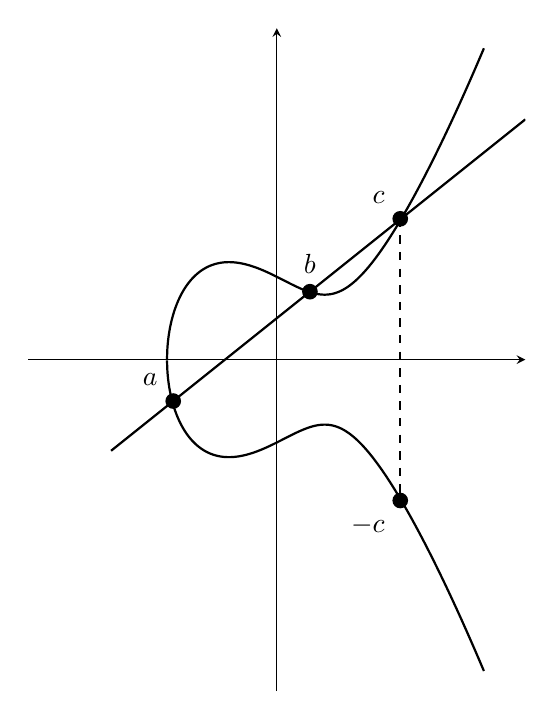
\begin{tikzpicture}
    \begin{axis}[
      axis lines=center,
      xlabel={},
      ylabel={},
      xmin=-3, xmax=3,
      ymin=-4, ymax=4,
      samples=100,
      smooth,
      width=10cm,
      height=10cm,
      axis equal image,
      ticks=none
    ]
    
    % Draw the elliptic curve: y^2 = x^3 - x + 1
    \addplot[
      domain=-2:2.5,
      thick,
      black,
      samples=2000
    ] ({x}, {sqrt(x^3 - x + 1)});
    
    \addplot[
      domain=-2:2.5,
      thick,
      black,
      samples=2000
    ] ({x}, {-sqrt(x^3 - x + 1)});

    % Draw the line through P, Q, and R
    \addplot[
      domain=-2:3,
      thick,
      black
    ] {0.8*x + 0.5};
    
    % Mark and label the points
    \node[circle, fill=black, inner sep=2pt, label=above left:$a$] at (axis cs:-1.25,-0.5) {};
    \node[circle, fill=black, inner sep=2pt, label=above:$b$] at (axis cs:0.4,0.82) {};
    \node[circle, fill=black, inner sep=2pt, label=above left:$c$] at (axis cs:1.49,1.70) {};
    \node[circle, fill=black, inner sep=2pt, label=below left:$-c$] at (axis cs:1.49,-1.70) {};
    \draw[dashed, thick, black] (axis cs:1.49,1.70) -- (axis cs:1.49,-1.70);
    
    \end{axis}
  \end{tikzpicture}
  \caption{Elliptic curve point addition and multiplication, with the curve $y^2 = x^3 - x + 1$.}
  \label{fig:elliptic-curve}
\end{figure}

What is the benefit of this? Its irreversibility. A private key is just a number; a public key is just that number multiplied by some other commonly agreed on number (the "base point") using elliptic curve arithmetic. Regular multiplication would mean that one could trivially obtain someone's private key by dividing their public key by the base point, but by bouncing all our operations around with elliptic curve multiplication, we prevent division.  This is less crude and more beautiful than it might seem, because these keypairs have some special properties that are useful for cryptography.

If Alice multiplies her private key by Bob's public key, \mbox{Alice} gets the same answer as if Bob multiplied his private key by Alice's public key. This allows the two parties to use that answer as a shared secret that only they know. In the \emph{Elliptic Curve Diffie-Hellman} (\ssc{ecdh}) protocol, we take the $x$ coordinate of that shared secret and run it through a key derivation function (in Urbit's case, \textsc{sha}-256) to get a symmetric key which allows them to both encrypt and decrypt messages. Using this key, they can communicate privately.

Similarly, \emph{Elliptic Curve Digital Signature Algorithm} (\ssc{ecdsa}) uses a more extensive algorithm to allow Alice to sign a message with her private key and for Bob to use his public key to verify that Alice did in fact sign it.

The elliptic curve that Urbit uses for key generation is the fast and
un-patented \emph{Curve25519}. This specifies the curve equation, the base point, and the finite field (the range of integers that we operate on, wrapping back to 0 if we go over the max value). There are two algebraically equivalent representations of Curve25519 that Urbit uses, with each defining its own set of standard operations: Montgomery Form (X25519), which is more efficient for \textsc{ecdh}, and Twisted Edwards Form (Ed25519), which is more efficient for \textsc{eddsa} (an elliptic curve signature scheme similar to \textsc{ecdsa}).

Urbit implements the Ed25519 standard operations in its
\lstinline[style=inlinecode]{+ed:crypto} zuse core for \textsc{eddsa}, along with a few X25519-like
operations for \textsc{ecdh}.

\begin{itemize}
  \item  \lstinline[style=inlinecode]{+scam}: scalar multiply. Takes a point and a scalar → returns scalar × point. This is the core elliptic curve operation.
  \item  \lstinline[style=inlinecode]{+ward}: point addition (Edwards curve formula). Needed for scalar multiplication by repeated doubling-and-adding.
  \item  \lstinline[style=inlinecode]{+etch}/\lstinline[style=inlinecode]{+deco}: encode/decode a curve point into/from an atom. This is how keys are serialized.
  \item  \lstinline[style=inlinecode]{+luck}: derive a keypair (public plus private) from a seed. This is how comets/\-planets get Curve25519 keys.
  \item  \lstinline[style=inlinecode]{+puck}: get the public key from a seed.
  \item  \lstinline[style=inlinecode]{+slar}/\lstinline[style=inlinecode]{+shar}: perform a Diffie--Hellman secret derivation (\textsc{ecdh}). Given your private scalar and someone else's public point, return a shared secret.
  \item  \lstinline[style=inlinecode]{+sign}/\lstinline[style=inlinecode]{+sign-raw}/\lstinline[style=inlinecode]{+sign-octs}: produce signatures. This is the \textsc{ecdsa}/\textsc{eddsa}-like functionality.
  \item  \lstinline[style=inlinecode]{+veri}/\lstinline[style=inlinecode]{+veri-octs}: verify signatures against a public key.
\end{itemize}

\noindent
With all of this context, you can imagine why we'd want to have two
pairs of networking keys: \textsc{ecdh} encryption and \mbox{\textsc{eddsa}} signatures are both complicated mathematical operations, so it's cleaner and safer to delineate between the two protocols completely in case of implementation bugs, future cryptographic discoveries, nonce reuse, and key rotations.

So how are these keypairs turned into an atom, where are they stored,
and when are they used?

\section{Asymmetric Cryptosuites}\label{asymmetric-cryptosuites}

The usage of public and private keys we've described so far is called
\emph{asymmetric cryptography}.  In current Arvo, the only existing implementation is \lstinline[style=inlinecode]{+crub:crypto} in zuse:

\begin{itemize}
  \item  \lstinline[style=inlinecode]{+seal}: encrypt to a peer. Runs \textsc{ecdh} with our encode secret plus their encode pubkey, hashes with \textsc{sha}-256, signs with our auth secret, encrypts with \textsc{aes}-\textsc{siv}.
  \item  \lstinline[style=inlinecode]{+sign}: sign a message with our auth secret (\textsc{eddsa}).
  \item  \lstinline[style=inlinecode]{+sure}: verify a message was signed with the matching auth pubkey.
  \item  \lstinline[style=inlinecode]{+tear}: decrypt from a peer. \textsc{ecdh} with our encrypt secret plus their encrypt pubkey, \textsc{sha}-256, \textsc{aes}-\textsc{siv} decrypt, then verify signature.
  \item  \lstinline[style=inlinecode]{+fig}: \textsc{sha}-256 fingerprint of the public key(s).
  \item  \lstinline[style=inlinecode]{+pac}: \textsc{sha}-256 fingerprint of the secret key(s).
  \item  \lstinline[style=inlinecode]{+pub}: concatenate encode pubkey plus auth pubkey into one atom.
  \item  \lstinline[style=inlinecode]{+sec}: concatenate encode secret plus auth secret into one atom.
  \item  \lstinline[style=inlinecode]{+pit}: generate a new keypair from a seed. Uses \textsc{sha}-512 for privates, \lstinline[style=inlinecode]{+puck:ed:crypto} for publics.
  \item  \lstinline[style=inlinecode]{+nol}: reconstruct a \lstinline[style=inlinecode]{+crub} from a secret key atom.
  \item  \lstinline[style=inlinecode]{+com}: reconstruct a \lstinline[style=inlinecode]{+crub} from a public key atom.
\end{itemize}

Here we have the key derivation and signing functions as wrappers around \lstinline[style=inlinecode]{+ed:crypto} and \lstinline[style=inlinecode]{+aes:crypto}, along with arms for turning networking keys into atoms and atoms back into \ldots{} \lstinline[style=inlinecode]{+crub}s? You'd think that we'd turn an atom back into a pair of networking keys. Right?

But what if you wanted to use a different cryptosuite with Ames? Then all of your old keys would be stranded as incompatible atoms. By using a \lstinline[style=inlinecode]{+crub} object instead, with keys in its payload and a battery for how to use them, we maintain consistency even if there were multiple implementations of \lstinline[style=inlinecode]{+acru}.

We do, then, need to track which cryptosuite to decode a key atom
to---so we store this in the Jael secrets vane right next to the keys themselves:

\begin{lstlisting}[style=listingblock]
+$  point
  $:  =rift
      =life
      keys=(map life [crypto-suite=@ud =pass])
      sponsor=(unit @p)
  ==
\end{lstlisting}

Now we can begin to home in on exactly what needs to change in the Urbit crypto suite in order for Groundwire to allow comets to rotate their keys.

\sloppy
In current Arvo (Listing~\ref{lst:arvo}), when a comet contacts another ship, that ship will ask the comet for an \emph{unecrypted self-attest\-ation packet} to prove that the sender does in fact control the private key whose public counterpart was hashed into the comet's \lstinline[style=inlinecode]{@p}.

But Groundwire comets don't self-attest to their identity; that
attestation comes into Jael via \lstinline[style=inlinecode]{%ord-watcher} in the same way that
Azimuth attestations come into Jael via \lstinline[style=inlinecode]{%azimuth} and \lstinline[style=inlinecode]{%eth-watcher}. In the Groundwire codebase, the \lstinline[style=inlinecode]{+request-} \lstinline[style=inlinecode]{attestation} arm is
replaced with (Listing~\ref{lst:groundwire}).

If we have this comet's networking keys in Jael (and thus \lstinline[style=inlinecode]{lyf} is not null), then instead of asking the comet to self-attest, we check our recorded networking keys. So far, so good: even though we're still expecting the comet's \lstinline[style=inlinecode]{@p} to match its public key in the non-Groundwire \lstinline[style=inlinecode]{?:} wutcol branch, we can skip that check and trust Jael for Groundwire comets. So why do we need to change our crypto suite?

\section{Tweaked Keys}\label{tweaked-keys}

Groundwire's proposed change to comet attestation has greater
philosophical implications for identity than you might expect.

Groundwire's strategy is to bet on Bitcoin being the one true long-term substrate that Urbit's \textsc{pki} will live on, because Bitcoin is the only chain that offers an unambiguous protocol-level definition of canonical history (``the longest valid proof-of-work chain'') that a zero-kelvin Urbit could resolve without appeal to social coordination or trusted checkpoints.

But it \emph{is} a bet, and a contentious one at that in an ecosystem
that includes Ethereum and Nockchain. For this reason, we \emph{don't} insist that Jael only ingest comet \textsc{pki} data from Bitcoin.

All of Groundwire's changes to Arvo stem from modifying Ames's
\lstinline[style=inlinecode]{+request-attestation} arm to \lstinline[style=inlinecode]{+fetch-comet-pki}, with the core proposition being that comets have the ability to publish their networking keys to any source of \textsc{pki} truth that other Urbit ships choose to interpret. To enable this, comets need to somehow encode within Jael \emph{which} \textsc{pki} they've attested to. This is where tweaked keys come in.

The payload of \lstinline[style=inlinecode]{+crub} is:

\begin{lstlisting}[style=listingblock]
[pub=[cry=@ sgn=@] sek=(unit [cry=@ sgn=@])]
\end{lstlisting}

\noindent
which are an encryption public key, a signing public key, and optionally their secret counterparts.

The Groundwire codebase introduces a new crypto-suite, \lstinline[style=inlinecode]{+cric}, with the payload:

\begin{lstlisting}[style=listingblock]
$%  $:  suite=%b
        pub=[cry=@ sgn=@ ~]
        sek=$@(~ [sed=@ cry=@ sgn=@])
    ==
    $:  suite=%c
        pub=[cry=@ sgn=@ tw=[ugn=@ dat=@]]
        sek=$@(~ [sed=@ cry=@ sgn=@])
==  ==
\end{lstlisting}

\begin{lstlisting}[style=listingcode,caption={The current Arvo comet handler.},label={lst:arvo}, float={!p}]
::  +request-attestation: helper to request
::  attestation from comet. Also sets a timer
::  to resend the request every 30s.
::
++  request-attestation
  |=  =ship
  ^+  event-core
  =+  %^    ev-trace
          msg.veb
        ship
      |.("requesting attestion")
  =.  event-core
    =/  =blob  (sendkeys-packet ship)
    %:  send-blob
        for=|
        ship
        blob
        (~(get by peers.ames-state) ship)
    ==
  =/  =wire  /alien/(scot %p ship)
  (emit duct %pass wire %b %wait (add now ~s30))
\end{lstlisting}

\begin{lstlisting}[style=listingcode,caption={The current Groundwire comet handler.},label={lst:groundwire}, float={!p}]
++  fetch-comet-pki
  |=  =ship
  ^+  event-core
  =+  %^    ev-trace
          msg.veb
        ship
      |.("requesting attestion")
  =/  lyf
    %:  rof
        [~ ~]
        /ames
        %j
        `beam`[[our %lyfe %da now] /(scot %p ship)]
    ==
  ?:  ?=([~ ~ [* * ^]] lyf)
    =.  event-core  (emil moves)
    %-  emit
      :*  [//keys]~
          %pass
          /public-keys
          %j
          %public-keys
          ship
          ~
          ~
      ==
  =.  event-core
    =/  =blob  (sendkeys-packet ship)
    %:  send-blob
        for=|
        ship
        blob
        (~(get by peers.ames-state) ship)
    ==
  =/  =wire  /alien/(scot %p ship)
  (emit duct %pass wire %b %wait (add now ~s30))
\end{lstlisting}

\newpage
\noindent
We refer to \lstinline[style=inlinecode]{+crub} as ``Suite B'' because it implements the \textsc{nsa} Suite B Cryptography Standard. \lstinline[style=inlinecode]{+cric} includes everything in Suite B, along with a new ``Suite C'' (a coinage of our own).

The Suite C payload's main difference is that the signing keys are ``tweaked''. We store \lstinline[style=inlinecode]{ugn}, the untweaked public key, and \lstinline[style=inlinecode]{sed}, the random seed used to originally generate our untweaked keypair, so that we have everything we need to recreate them if we ever need to. Then, we can tweak them by passing them into a tweaking function along with a bytestring, \lstinline[style=inlinecode]{dat} (omitting from our tweak the additional new field \lstinline[style=inlinecode]{xtr} which can include extra data):

\begin{lstlisting}[style=listingblock]
::  pub.s = public signing key
::  sek.s = private signing key
=/  mit
  (shax (can 3 [32 pub.s] [(met 3 dat) dat] ~))
(scad:ed pub.s sek.s mit)
\end{lstlisting}

First, the public key is hashed along with the data to produce \lstinline[style=inlinecode]{mit}, the ``tweak scalar.'' All three of these arguments get passed into \lstinline[style=inlinecode]{+scad:ed}, a wrapper around two other \lstinline[style=inlinecode]{+ed} arms:

\begin{lstlisting}[style=listingblock]
::  scalar addition on public and private keys
++  scad
  ~/  %scad
  |=  [pub=@uxpoint sek=@uxscalar sca=@uxscalar]
  ^-  [pub=@uxpoint sek=@uxscalar]
  [(scap pub sca) (scas sek sca)]
\end{lstlisting}

\noindent
These two arms, \lstinline[style=inlinecode]{+scap} and \lstinline[style=inlinecode]{+scas}, perform elliptic curve addition between the tweak scalar and corresponding key.

Anyone with both your public untweaked key and your tweak data can
recreate your tweaked key. And, sure enough, we recall the
\lstinline[style=inlinecode]{$point:jael} type:

\begin{lstlisting}[style=listingblock]
+$  point
  $:  =rift
      =life
      keys=(map life [crypto-suite=@ud =pass])
      sponsor=(unit @p)
  ==
\end{lstlisting}

\noindent
wherein the \lstinline[style=inlinecode]{pass} field is the atom that, in Suite B, encodes the two public keys. In Suite C, it encodes the encryption key, the untweaked signing key, \emph{and} the tweak data. Upon receiving a message from a comet, your ship can reconstruct the tweaked key and check if it matches the key that the comet provides.

This might seem like a ton of unnecessary work. If you already trust Jael's sources of truth (\lstinline[style=inlinecode]{%ord-watcher}, in this case), why bother with tweaked keys at all?

The reason is that tweaking keys allows for a bidirectional cryptographic commitment between on-chain and off-chain attestations to prevent replay, spoofing, and double-spawning attacks. If there wasn't an off-chain anchor pointing to on-chain data, then anyone could come in and attest to ownership of any comet and \lstinline[style=inlinecode]{%ord-watcher} would naively believe them.

In Groundwire's implementation, that anchor is the ordinal number of the sat used for the comet's inscription. When \lstinline[style=inlinecode]{%ord-watcher} sees an attempted key rotation, it checks the specified comet identity's \lstinline[style=inlinecode]{$pass} in Jael to verify that the transaction's ordinal number matches the current tweak data, and rejects it if it doesn't. Back in userspace, any agent can later recompute the tweak to confirm that the key they're communicating with really does originate from the expected on-chain inscription.

This tweaked key protocol enables a new conception of identity on Urbit: rift, life, keys, \emph{and data}.

\section{Routing}\label{routing}

The final implication of Groundwire's change to Ames' interpretation of comet provenance is that, since Groundwire comets articulate a network independent of Azimuth, they shouldn't need to rely on the current sponsorship hierarchy for packet routing. To facilitate this, comets can include include another piece of info in their attestations, called a \lstinline[style=inlinecode]{$fief}:

\begin{lstlisting}[style=listingblock]
+$  fief
  $%  [%turf p=(list turf) q=@udE]
      [%if p=@ifF q=@udE]
      [%is p=@isH q=@udE]
  ==
\end{lstlisting}

\noindent
in which \lstinline[style=inlinecode]{$point:jael} is updated to contain a \lstinline[style=inlinecode]{(unit fief)}, potentially storing the comet's static IP address (\lstinline[style=inlinecode]{%if} for IPv4 or \lstinline[style=inlinecode]{%is} for IPv6) or domain (\lstinline[style=inlinecode]{%turf}).

On top of this, Ames has been updated to allow any ship to be a valid
sponsor, necessitating a few changes to its routing logic to detect
cycles and ensure that sponsorship chains are allowed to terminate in
any sponsor with a \lstinline[style=inlinecode]{$fief}, rather than only in galaxies.\tombstone

\selectlanguage{USenglish}
% \printbibliography
\end{document}
